\section*{Oppgave 1 - Interpolated Precision}
\vspace{200pt}
\begin{minipage}[t]{.25\linewidth}
\vspace{0pt}
\centering
    \begin{tabular}{| l | l |}
    \hline
    RL & IP \\ \hline
    0.0 & 1 \\ \hline
    0.1 & 1 \\ \hline
    0.2 & 0.66 \\ \hline
    0.3 & 0.66 \\ \hline
    0.4 & 0.5 \\ \hline
    0.5 & 0.5 \\ \hline
    0.6 & 0.45 \\ \hline
    0.7 & 0.45 \\ \hline
    0.8 & 0.45 \\ \hline
    0.9 & 0.0 \\ \hline
    1.0 & 0.0 \\ \hline
    \end{tabular}
\end{minipage}%
\begin{minipage}[t]{.25\linewidth}
\vspace{0pt}
\centering
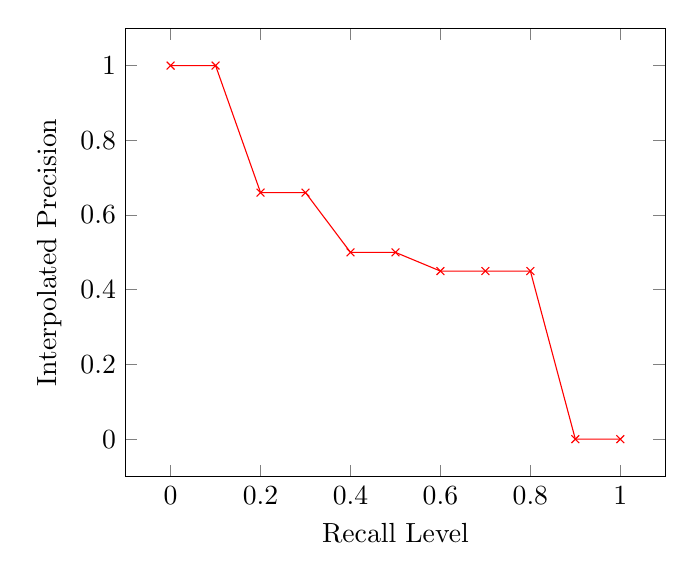
\begin{tikzpicture}
	\begin{axis}[
		xlabel=Recall Level,
		ylabel=Interpolated Precision]
	\addplot[color=red,mark=x] coordinates {
		(0.0,1)
		(0.1,1)
		(0.2,0.66)
		(0.3,0.66)
		(0.4,0.5)
		(0.5,0.5)
		(0.6,0.45)
		(0.7,0.45)
		(0.8,0.45)
		(0.9,0.0)
		(1.0,0.0)
		
	};
	\end{axis}
\end{tikzpicture}
\end{minipage}